\documentclass[a4paper, 12pt]{article}

% Essential Packages
\usepackage{amsmath}
\usepackage{amssymb}
\usepackage[top=25mm, bottom=25mm, left=25mm, right=25mm]{geometry}
\usepackage{pgfplots}
\usepackage[inline]{enumitem}
\usepackage{mathtools}
\usepackage{tikz}
\usepackage{fancyhdr}
\usepackage{setspace}
\usepackage{hyperref}

% Misc
\pgfplotsset{compat=1.18}
\usepgfplotslibrary{polar}
\usepgfplotslibrary{fillbetween}
\setlength{\parskip}{3pt}
\setstretch{1.15}
\renewcommand{\headrulewidth}{0pt}
\renewcommand{\footrulewidth}{0pt}
\fancyhf{}

\begin{document}
\pagestyle{empty}

\begin{center}
\textbf{2011-2012 Spring \\MAT123 Midterm II\\08/05/2012\\Duration: 105 minutes}
\end{center}

\begin{enumerate}[leftmargin=*,label=\textbf{\arabic*.}]
\item Consider the region bounded by the curve $y=x^2$, the $x$-axis, and the line $x=2$, where $x\geq0$.

\begin{enumerate}[leftmargin=*,label=\textbf{\alph*.}]
\item Find the volume of the solid generated by revolving the region about the $x$-axis by the disk method and sketch the solid.
\item Find the volume of the solid generated by revolving the region about the $y$-axis by the shell method and sketch the solid.
\end{enumerate}

\item Evaluate the following integrals.

\begin{enumerate}[leftmargin=*,label=\textbf{\alph*.}]
\item $\displaystyle \int_0^3\left|x^2-1\right|\, dx$
\item $\displaystyle\int\frac1{x^2+2x+1}\,dx$
\item $\displaystyle\int\frac1{x^2+2x+2}\,dx$
\item $\displaystyle\int\frac1{x^2+3x+2}\,dx$
\item $\displaystyle\int_{-\pi/6}^0\sqrt{1-\cos(6x)}\,dx$
\end{enumerate}

\item Determine whether the improper integral $\displaystyle\int_{-\infty}^\infty\frac1{1+x^2}\,dx$ is convergent or divergent. Evaluate if the integral is convergent.

\item Evaluate the following limits. Explain all your work and write clearly.

\begin{enumerate}[leftmargin=*,label=\textbf{\alph*.}]
\item $\displaystyle\lim_{x\to0}\frac{3^x-1}{5^x-1}$
\item $\displaystyle \lim_{x\to0}\frac{\displaystyle\int_0^{x^2}\sin t\,dt}x$
\end{enumerate}

\item Determine whether each sequence converges or diverges. Evaluate the limit of each convergent sequence. Explain all your work and write clearly.

\begin{enumerate}[leftmargin=*,label=\textbf{\alph*.}]
\item $\displaystyle a_n=\frac{2n+(-1)^n}n$
\item $\displaystyle a_n=\arctan\left(\frac{n+1}n\right)$
\item $\displaystyle a_n = \frac{n+1}{1-\sqrt n}$
\end{enumerate}
\end{enumerate}

\newpage
\pagestyle{fancy}
\renewcommand{\headrulewidth}{1pt}
\fancyhead[R]{\textit{2011-2012 Spring Midterm II}}
\fancyhead[L]{\textit{Hacettepe MAT123 Exam Solutions Version 2}}

% Last update: 29/08/2025 20:11

\begin{enumerate}[leftmargin=*,label=\textbf{\arabic*.}]

\item\leavevmode
\vspace{-1.5em}
\begin{center}
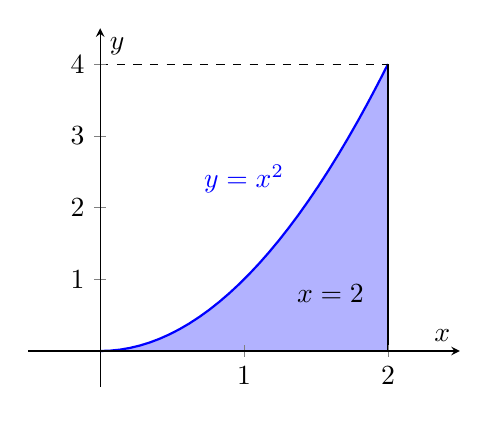
\begin{tikzpicture}
  \begin{axis}[
    axis lines=middle,
    xmin=-0.5, xmax=2.5,
    ymin=-0.5, ymax=4.5,
    xtick={0,1,2},
    ytick={0,1,2,3,4},
    xlabel=$x$, ylabel=$y$,
    domain=0:2,
    samples=30,
    axis on top,
    clip=true,
    scale=0.8,
    ]
    
    \addplot [
      draw=none,
      fill=blue!30,
    ]
    {x^2}
    \closedcycle;

    \addplot [thick, blue] {x^2};

    \draw (axis cs:2,0) -- (axis cs:2,4);
    \draw[dashed] (axis cs:0,4) -- (axis cs:2,4);
    \node[blue] at (1,2.4) {$y=x^2$};
    \node at (1.6,0.8) {$x=2$};
   \end{axis}
\end{tikzpicture}
\end{center}

\begin{enumerate}[leftmargin=*,label=\textbf{\alph*.}]

\item\leavevmode
\vspace{-1em}
\begin{center}
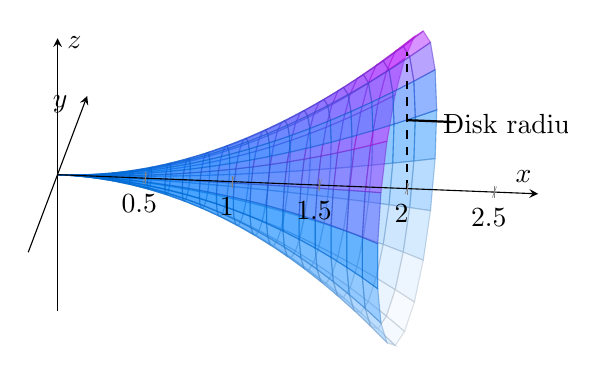
\begin{tikzpicture}
  \begin{axis}[
    view={7}{30},
    axis on top,
    axis lines=middle,
    xlabel={$x$},
    ylabel={$y$},
    zlabel={$z$},
    ytick={-4,4}, ztick={-4,4},
    samples=20,
    xmin=0, xmax=2.75,
    domain=0:2,
    y domain=0:360,
    colormap/cool,
    scale=1.,
    ytick=\empty, ztick=\empty
    ]
    
    \addplot3 [
      surf,
      opacity=0.5,
    ]
    (
      x,
      {x^2 * cos(y)},
      {x^2 * sin(y)}
    );

    \draw[dashed, thick] (2,0,0)--(2,0,4);
    \draw[thick] (2,0,2)--(2.28,0,2);

    \node at (2.6,0,2) {Disk radius};
  \end{axis}
\end{tikzpicture}
\end{center}
\begin{align*}
\text{Volume}&=\int_{\mathcal{D}}\pi\cdot(r(x))^2\,dx=\int_0^2\pi\left(x^2\right)^2\,dx=\pi\int_0^2x^4\,dx=\pi\left[\frac{x^5}5\right]_0^2=\boxed{\frac{32\pi}5}
\end{align*}

\item\leavevmode
\vspace{-1em}
\begin{center}
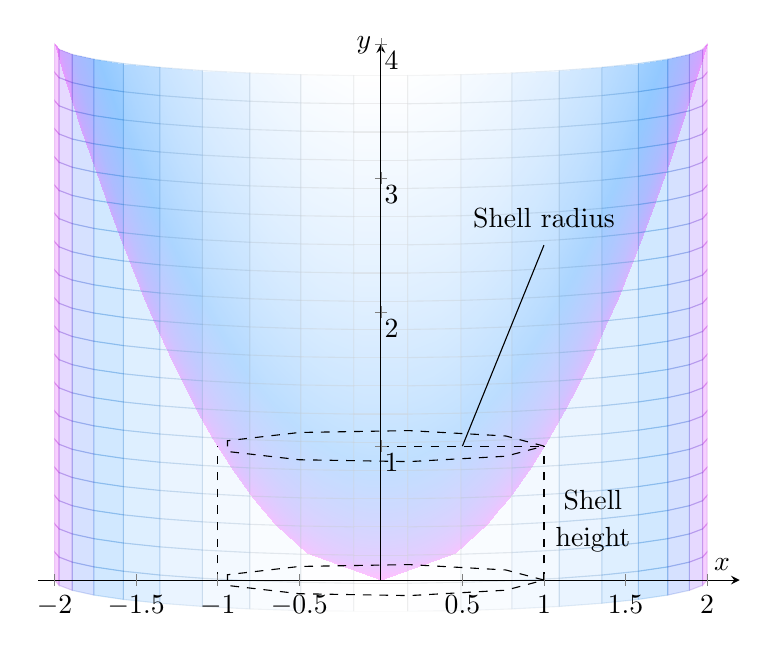
\begin{tikzpicture}
  \begin{axis}[
  view={0}{85},
    axis lines=center,
    axis on top,
    xlabel={$x$},
    ylabel={$y$},
    zlabel={$z$},
    hide z axis,
    xmin=-2.1, xmax=2.2,
    samples=20,
    domain=0:4,
    y domain=180:360,
    colormap/cool,
    scale=1.3,
    ]

    \addplot3 [
      surf,
      opacity=0.3,
      shader=interp,
    ]
    (
      {sqrt(x) * cos(y)},
      {x},
      {sqrt(x) * sin(y)}
    );
    
    \addplot3[
      surf,
      opacity=0.2,
    ]
    (
      {2 * cos(y)},
      {x},
      {2 * sin(y)}
    );

    \addplot3[
      domain=0:360,
      samples=10,
      dashed,
    ]
    (
      {cos(x)},
      {1},
      {sin(x)}
    );
    
    \addplot3[
      domain=0:360,
      samples=10,
      dashed,
    ]
    (
      {cos(x)},
      {0},
      {sin(x)}
    );
    \draw[dashed] (1,0,0)--(1,1,0);
    \draw[dashed] (-1,0,0)--(-1,1,0);
    \draw[dashed] (0,1,0)--(1,1,0);
    \draw (0.5,1,0)--(1,2.5,0);
    \node at (1.3,0.6,0) {Shell};
    \node at (1.3,0.3,0) {height};
    \node at (1,2.7,0) {Shell radius};
  \end{axis}
\end{tikzpicture}
\end{center}
\begin{align*}
\text{Volume}&=\int_{\mathcal{D}}2\pi\cdot r(x)\cdot h(x)\,dx=2\pi\int_0^2x\cdot x^2\,dx=2\pi\int_0^2x^3\,dx\\[1em]&=2\pi\left[\frac{x^4}4\right]_0^2=2\pi\left(\frac{2^4}4-0\right)=\boxed{8\pi}
\end{align*}
\end{enumerate}

\item \begin{enumerate}[leftmargin=*,label=\textbf{\alph*.}]

\item The expression $\left|x^2-1\right|$ is the same as $x^2-1$ for $x>1$ and $1-x^2$ for $x<1$. We can write the equivalent expression below.
\begin{align*}\int_0^3\left|x^2-1\right|&=\,dx\int_0^1\left(1-x^2\right)\,dx+\int_1^3(x^2-1)\,dx=\left[x-\frac{x^3}3\right]_0^1+\left[\frac{x^3}3-x\right]_1^3\\[1em]&=\left[\left(1-\frac{1^3}3\right)-0\right]+\left[\left(\frac{3^3}3-3\right)-\left(\frac{1^3}3-1\right)\right]=\boxed{\frac{22}3}\end{align*}

\item $\displaystyle\int\frac1{x^2+2x+1}\,dx=\int\frac1{(x+1)^2}\,dx=\boxed{-\frac1{x+1}+c, \quad c\in\mathbb{R}}$

\item Rewrite the integrand.
\begin{align*}\int\frac1{x^2+2x+2}\,dx&=\int\frac1{(x+1)^2+1}\,dx\quad\left[u=x+1\implies du=dx\right]\\[1em]&=\int\frac1{u^2+1}\,du=\arctan(u)+c=\boxed{\arctan(x+1) +c,\quad c\in\mathbb{R}}\end{align*}

\item We can use the method of partial fraction decomposition.

\begin{equation}\int\frac1{x^2+3x+2}\,dx=\int\frac1{(x+1)(x+2)}\,dx=\int\left(\frac A{x+1}+\frac B{x+2}\right)\,dx\label{eq:11_12_spring_midterm2_1}\end{equation}

Expand the numerator.
\begin{align*}
A(x+2)+B(x+1)&=1\\
x(A+B)+2A+B&=1\\
\therefore A+B=0\quad[\text{eliminate}\ x]\,&\rightarrow\,2A+B=1
\end{align*}

Solve for $A$ and $B$.
\[
\left.
\begin{array}{ll}
A+B=0\\
\displaystyle2A+B=1
\end{array}
\right\}
\quad A=1,\quad B=-1
\]

Plug the values of $A$ and $B$ into \eqref{eq:11_12_spring_midterm2_1}.
\begin{align*}
\int\left(\frac{A}{x+1}+\frac{B}{x+2}\right)\,dx
&= \int\left(\frac{1}{x+1}-\frac{1}{x+2}\right)\,dx \\[1em]
&= \boxed{\ln\left|x+1\right|-\ln\left|x+2\right|+c,\quad c\in\mathbb{R}}
\end{align*}

\item Use the trigonometric identity $\cos(2x)=1-2\sin^2x$.
\[\int_{-\pi/6}^0\sqrt{1-\cos(6x)}\,dx=\int_{-\pi/6}^0\sqrt{2\sin^2(3x)}\,dx=\sqrt2\int_{-\pi/6}^0\left|\sin(3x)\right|\,dx\]

$\sin x<0$ for $-\pi<x<\pi$. Therefore, the integral can be rewritten as follows.
\begin{align*}\sqrt2\int_{-\pi/6}^0\left|\sin(3x)\right|\,dx&=\sqrt2\int_{-\pi/6}^0-\sin(3x)\,dx=\sqrt2\left[\frac13\cos(3x)\right]_{-\pi/6}^0\\[1em]&=\frac{\sqrt2}3\left[\cos0-\cos\left(-\frac\pi2\right)\right]=\boxed{\frac{\sqrt2}3}\end{align*}
\end{enumerate}

\item We have an improper integral where the limits are $\pm\infty$. Use limits to handle improper integrals accurately.
\begin{align*}
\int_{-\infty}^\infty\frac1{1+x^2}\,dx&=\lim_{A\to\infty}\int_{-A}^A\frac1{1+x^2}\,dx = \lim_{A\to\infty}\arctan(x)\bigg|_{-A}^A\\[1em]&=\lim_{A\to\infty}\left(\arctan A-\arctan(-A)\right)=\frac\pi2-\left(-\frac\pi2\right)=\boxed\pi
\end{align*}

The value of the improper integral is finite. Therefore, this integral is convergent.

\item \begin{enumerate}[leftmargin=*,label=\textbf{\alph*.}]
\item The limit is in the indeterminate form $0/0$. We can apply L'Hôpital's rule to eliminate the indeterminate form.
\[\lim_{x\to0}\frac{3^x-1}{5^x-1}\overset{\text{L'H.}}{=}\lim_{x\to0}\frac{3^x\cdot\ln3}{5^x\cdot\ln5}=\log_53\cdot\lim_{x\to0}\left(\frac35\right)^x=\boxed{\log_53}\]

\item The first method is to evaluate the integral in the limit.
\[\lim_{x\to0}\frac{\displaystyle\int_0^{x^2}\sin t\,dt}x=\lim_{x\to0} \frac{-\cos t\,\bigg|_{t=0}^{t=x^2}}x=\lim_{x\to0}\frac{-\cos x^2-(-\cos0)}x=\lim_{x\to0}\frac{1-\cos x^2}x\]

Multiply by the expression inside the limit $\displaystyle \frac xx$. Notice that we obtain a standard form.
\begin{align*}\lim_{x\to0}\left(\frac{1-\cos x^2}x\cdot\frac xx\right)&=\lim_{x\to0}\frac{1-\cos x^2}{x^2}\cdot\lim_{x\to0}x\quad\left[\lim_{u\to0}\frac{1-\cos u}u = 0\right]\\[1em]&=0\cdot0=\boxed0\end{align*}

The second method is to use L'Hôpital's rule because of the $0/0$ form.
\[\lim_{x\to0}\frac{\displaystyle\int_0^{x^2}\sin t\,dt}x\overset{\text{L'H.}}{=}\lim_{x\to0}\frac{\displaystyle\frac d{dx}\int_0^{x^2}\sin t\,dt}1\]

Let $u=x^2$, then $du=2x\,dx$. By the Fundamental Theorem of Calculus, the limit can be rewritten as follows.
\begin{align*}
\lim_{x\to0}\frac{d}{dx}\int_0^{x^2}\sin t\,dt
&= \lim_{x\to0}\frac{d}{du}\left(\int_0^u\sin t\,dt\right)\frac{du}{dx} \\[1em]
&= \lim_{x\to0}\left(\sin u\cdot2x\right)
 = \lim_{x\to0}\left[2x\sin\left(x^2\right)\right]
 = \boxed{0}
\end{align*}
\end{enumerate}

\item \begin{enumerate}[leftmargin=*,label=\textbf{\alph*.}]
\item Rewrite the sequence.
\[a_n=\frac{2n+(-1)^n}{n}=2+\frac{(-1)^n}n\]

The sequence converges to $\boxed2$ because $\displaystyle\frac{(-1)^n}n\to 0$ as $n\to\infty$.
\item $\arctan(x)$ is continuous everywhere. Therefore, we can take the limit inside the expression.
\[\lim_{n\to\infty}\arctan\left(\frac{n+1}n\right)=\arctan\lim_{n\to\infty}\left(1+\frac1n\right)=\arctan1=\frac\pi4\]

The sequence converges to $\displaystyle\boxed{\frac\pi4}$.
\item Rewrite the sequence.
\[\lim_{n\to\infty}\frac{n+1}{1-\sqrt n}=\lim_{n\to\infty}\frac{\sqrt n\left(\sqrt n+\frac1{\sqrt n}\right)}{\sqrt n\left(\frac1{\sqrt n}-1\right)}=\lim_{n\to\infty}\frac{\sqrt n+\frac1{\sqrt n}}{\frac1{\sqrt n}-1}=-\infty\]

Notice that the denominator approaches $-1$ as $n\to\infty$ and the numerator approaches $\infty$ as $n\to\infty$. The sequence diverges to $\boxed{-\infty}$.
\end{enumerate}
\end{enumerate}
\end{document}